
\begin{frame}{}
    \begin{center}
        \large \textbf{ELMo: Embeddings from Language Models}
    \end{center}
    \vspace{20pt}
    
    \textbf{Author(s):}
    \begin{itemizeSpaced}{5pt}
    {\color{DimGrey} 
        \item Peters et al. (2018) in \emph{Deep Contextualized Word Representations}
        
    }
    \end{itemizeSpaced}
\end{frame}

% -------------------------------------------------



\begin{frame}{ELMo: Motivation}
    \footnotesize  
    
    Remember \textbf{polysemy}? \newline 
    
    ELMo makes contextual embeddings of a word according to its senses, so that ...
    
    \begin{exampleBlock}{Example}
        ... homonyms ``book" (text) and ``book" (reservation) get different vectors, not different meanings collapsed in one vector...\newline 
        
        Better than Word2Vec and GloVe!
        
    \end{exampleBlock}
    
    
    
\end{frame}



\begin{frame}{ELMo: Structure}
    \vspace{20pt}
    \begin{itemizeSpaced}{2pt}
        \pinkbox \textbf{ELMo} uses bidirectional language model (biLM) to make \emph{deep} word embeddings (derived from all its internal layers)

        \pinkbox Higher-level LSTM layers capture contextual meaning (useful for supervised word sense disambiguation (WSD)).
        
        \pinkbox Lower layers capture syntax information (useful for part of speech tagging (POS)). 
        
        \item \textbf{Task-Specific: } ELMo mixes the layers' signals in task-specific way: \footnotemark 
        $$
        \textbf{ELMo}_k^{task} = E \Big( R_k; \theta^{task} \Big) = \gamma^{task} \; \sum_{j=0}^L s_j^{task} \; \mathbf{h}_{kj}^{LM}
        $$ 
        
        \item ELMo embeddings are thus richer than traditional word vectors. 
    \end{itemizeSpaced}
    
    \footnotetext[1]{ the vector $\mathbf{s}^{task} = \Big\{ s_j^{task} \Big\}$ of softmax-normalized weights and task-dependent scalar parameter $\gamma^{task}$ allow the model for the specific $task$ to scale the entire $\textbf{ELMo}_k^{task}$ vector. The index $k$ corresponds to a $k$-th word, and index $j$ corresponds to the $j$-th layer out of $L$ layers. Here, $h_{kj}^{LM}$ is the output of the $j$-th LSTM for word $k$, and $s_j$ is the weight of $h_{kj}^{LM}$ used to compute the representation for word $k$. }
    
    
\end{frame}



\begin{frame}{ELMo: Strengths in POS Tagging and Word Sense Disambiguation}
    
    \vspace{10pt}
    
    \begin{table}[ht!]
      \centering
      \begin{tabular}{ c }
        
        \begin{minipage}{.9\textwidth}
          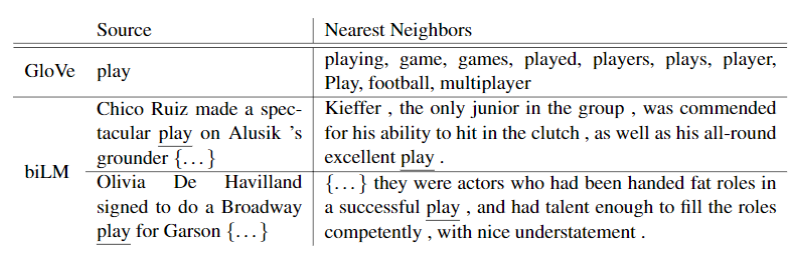
\includegraphics[width=\linewidth]{imgs/table_elmoPlay.png}
        \end{minipage}
        %\vspace{-7pt}
      \end{tabular}
      \caption{\linespread{0.3} \scriptsize Nearest neighbors to ``play” found by GloVe and biLM context embeddings. From \emph{Table 4 in Deep Contextualized Word Representations}, by Peters et al., 2018. \url{https://arxiv.org/pdf/1802.05365.pdf}. Copyright 2018 by Peters et al.}
      \label{tbl:elmoPlayExample}
      \vspace{-10pt}
    \end{table}
    
    \vspace{-15pt}
    
    \begin{itemizeSpaced}{5pt}
        
        \pinkbox GloVe's neighbors have different parts of speech, like verbs (``played", ``playing"), and nouns (``player", ``game") and only in the sport sense.
        
        
        \pinkbox biLM's nearest neighbor sentences from ``play'' CWE show clear difference between \emph{both} the parts of speech \emph{and} word sense of ``play". 
        
        \begin{itemizeSpaced}{0pt}
            \pinkbox last row: input sentence has noun / acting sense of ``play" and this is matched in the nearest neighbor sentence
        \end{itemizeSpaced}        
            
    
    \end{itemizeSpaced} 
    
    %\textbf{ELMo key feature: } learn context using part of speech tagging (POS) and word sense disambiguation (WSD).  
    
\end{frame}